
%%%%%%%%%%%%%%%%%%%%%
\section{Propriétés}
%%%%%%%%%%%%%%%%%%%%%

\subsection{Transformation de Lorentz}

\subsection{Relativité du mouvement}

\subsection{Exemple}
Un cycliste lache une balle. L'évenement $E_0$ : "lacher de la balle" se produit à une certaine date et à une certaine position dans le référentiel terrestre. Un second évenement, $E_1$ : "la balle touche une première fois le sol", se produit à une certaine date et à une certaine position.

\begin{center}
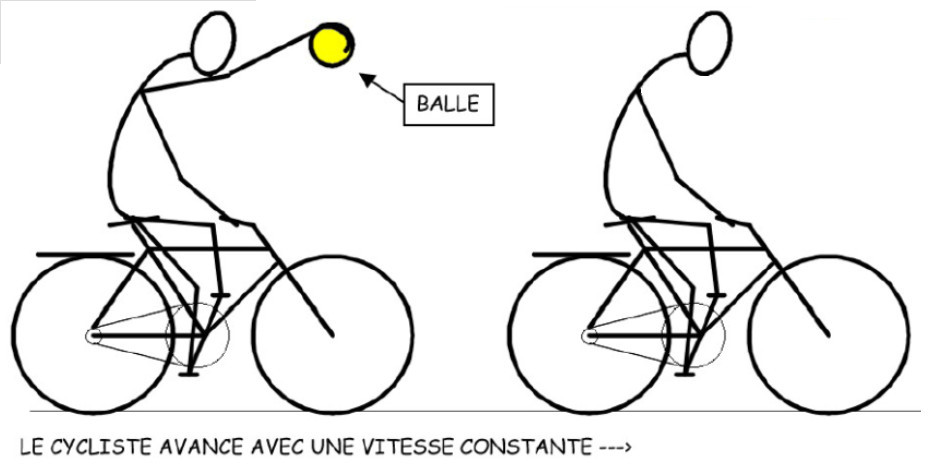
\includegraphics[scale=0.3]{./relativite/veloballe}
\end{center}

Sur le schéma, le vélo et le cycliste sont représentés deux fois : à la date de l'évenement $E_0$ et à celle de $E_1$. La balle n'est représentée qu'à la date de $E_0$.

La date de $E_1$ est déterminée par l'instant où la balle touche le sol. La position de la balle à ce moment là est à déterminer.

\subsection{Relativité de la simultanéïté}

% $E_1$
%
%%%%%%%%%%%%%%%%%%%%%%%%%%%%%%%%%%%%%%%%%%%%%%%%%%%%%%%%%%%%%%%%%%%%%%%%%%%%%%%%%%%%%
